\documentclass[11pt,a4paper]{article}

% ============================================================================
% PREAMBLE
% ============================================================================

\usepackage[utf8]{inputenc}
\usepackage[T1]{fontenc}
\usepackage{lmodern}
\usepackage[margin=0.65in]{geometry}
\usepackage[table]{xcolor}
\usepackage{tikz}
\usetikzlibrary{arrows.meta,positioning,shapes.geometric,calc,decorations.pathreplacing}
\usepackage{enumitem}
\usepackage{tabularx}
\usepackage{booktabs}
\usepackage{multicol}
\usepackage{graphicx}
\usepackage{amssymb}
\usepackage[colorlinks=true,linkcolor=ainblue,urlcolor=ainblue]{hyperref}

% Colors
\definecolor{ainblue}{RGB}{31,78,121}
\definecolor{aingray}{RGB}{89,89,89}
\definecolor{ainaccent}{RGB}{192,80,77}
\definecolor{aingreen}{RGB}{68,114,94}
\definecolor{ainlight}{RGB}{240,245,250}
\definecolor{aingold}{RGB}{180,140,50}
\definecolor{ainpurple}{RGB}{102,51,153}

% Page numbers
\pagestyle{plain}

% Custom commands
\newcommand{\ain}{\textsc{ain}}
\newcommand{\sectionline}{\noindent\makebox[\linewidth]{\color{ainblue}\rule{\textwidth}{0.8pt}}}

% Tight spacing
\setlength{\parskip}{0.35em}
\setlength{\parindent}{0pt}

% ============================================================================
% DOCUMENT
% ============================================================================

\begin{document}

% ----------------------------------------------------------------------------
% TITLE PAGE
% ----------------------------------------------------------------------------

\begin{center}
{\fontsize{48}{54}\selectfont\bfseries\color{ainblue} \ain}\\[0.4em]
{\LARGE\color{aingray} Where Ideas Prove Themselves}\\[1.2em]
{\large\itshape ``The forge where knowledge grows stronger.''}
\end{center}

\vspace{0.5em}
\sectionline
\vspace{0.3em}

% ----------------------------------------------------------------------------
% THE THREE-LAYER ARCHITECTURE
% ----------------------------------------------------------------------------

\begin{center}
{\Large\bfseries\color{ainblue} The Architecture: Three Layers}
\end{center}

\vspace{0.3em}

\begin{center}
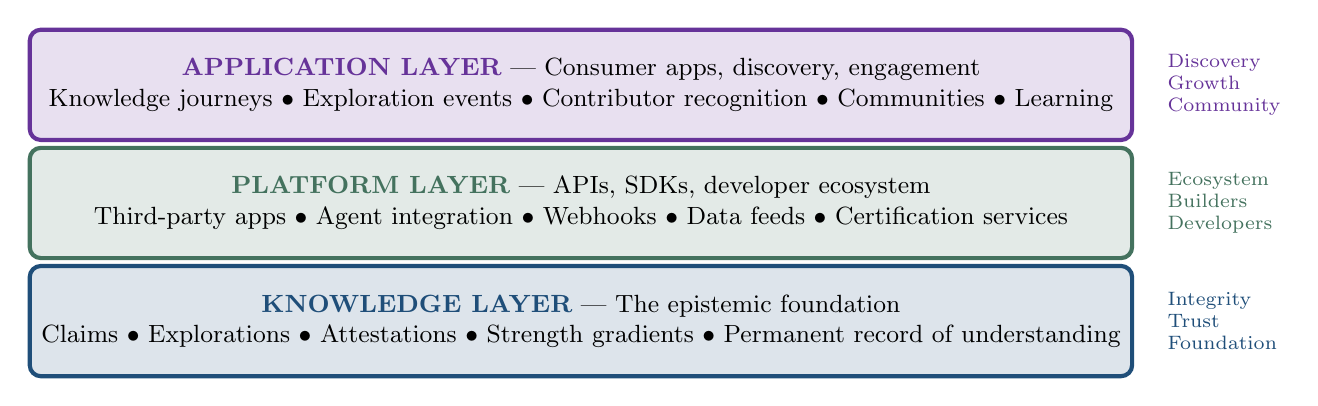
\begin{tikzpicture}[
    layer/.style={rectangle, rounded corners, draw=#1, line width=1.5pt, minimum width=14cm, minimum height=1.4cm, align=center, font=\small},
    arrow/.style={<->, thick, aingray, >=stealth}
]

% Layer 3 - Applications (top)
\node[layer=ainpurple, fill=ainpurple!15] (apps) at (0,3) {
    \textbf{\color{ainpurple}APPLICATION LAYER} --- Consumer apps, discovery, engagement\\
    \small Knowledge journeys $\bullet$ Exploration events $\bullet$ Contributor recognition $\bullet$ Communities $\bullet$ Learning
};

% Layer 2 - Platform (middle)
\node[layer=aingreen, fill=aingreen!15] (platform) at (0,1.5) {
    \textbf{\color{aingreen}PLATFORM LAYER} --- APIs, SDKs, developer ecosystem\\
    \small Third-party apps $\bullet$ Agent integration $\bullet$ Webhooks $\bullet$ Data feeds $\bullet$ Certification services
};

% Layer 1 - Truth (bottom)
\node[layer=ainblue, fill=ainblue!15] (truth) at (0,0) {
    \textbf{\color{ainblue}KNOWLEDGE LAYER} --- The epistemic foundation\\
    \small Claims $\bullet$ Explorations $\bullet$ Attestations $\bullet$ Strength gradients $\bullet$ Permanent record of understanding
};

% Annotations
\node[right=0.3cm of apps, font=\scriptsize, text=ainpurple, align=left] {Discovery\\Growth\\Community};
\node[right=0.3cm of platform, font=\scriptsize, text=aingreen, align=left] {Ecosystem\\Builders\\Developers};
\node[right=0.3cm of truth, font=\scriptsize, text=ainblue, align=left] {Integrity\\Trust\\Foundation};

% Bracket on left
% \draw[decorate, decoration={brace, amplitude=8pt, mirror}, thick, ainblue] 
%     (-7.5,-0.5) -- (-7.5,3.5) node[midway, left=10pt, align=right, font=\small] {\textbf{We own}\\the knowledge\\layer.\\\\Others build\\on top.};

\end{tikzpicture}
\end{center}

\vspace{0.3em}

\begin{center}
\colorbox{ainblue}{%
\begin{minipage}{0.95\textwidth}
\centering
\vspace{0.5em}
{\large\bfseries\color{white} The Platform Play}\\[0.3em]
{\color{white} 
The \textbf{Knowledge Layer} is the foundation: rigorous, trusted, incorruptible.\\
The \textbf{Platform Layer} lets anyone build on it: developers, enterprises, AI agents.\\
The \textbf{Application Layer} makes discovery engaging and growth visible.\\[0.3em]
\textbf{This is iOS for knowledge.} We provide the foundation. The world builds on top.
}
\vspace{0.5em}
\end{minipage}%
}
\end{center}

\sectionline

% ----------------------------------------------------------------------------
% THE KNOWLEDGE LAYER
% ----------------------------------------------------------------------------

\begin{center}
{\Large\bfseries\color{ainblue} Layer 1: The Knowledge Layer (The Foundation)}
\end{center}

\vspace{0.2em}

\begin{multicols}{2}

\textbf{What It Is:}
\begin{itemize}[nosep, leftmargin=1em]
    \item Claims, explorations, attestations, resolutions
    \item Cryptographically signed, content-addressed
    \item Permanent record of how ideas evolved
    \item \textbf{Strength gradients}: how thoroughly tested, how resilient
    \item Popper realized: knowledge through rigorous examination
\end{itemize}

\textbf{Properties (Inviolable):}
\begin{itemize}[nosep, leftmargin=1em]
    \item No rankings for sale
    \item No outcomes for sale
    \item No engagement manipulation
    \item Money funds \textit{exploration}, not \textit{results}
    \item Forkable if ever compromised
\end{itemize}

\columnbreak

\textbf{Why It's Valuable:}
\begin{itemize}[nosep, leftmargin=1em]
    \item Only source of rigorously-tested knowledge
    \item Gradients reflect genuine examination and resilience
    \item Institutional-grade epistemic infrastructure
    \item Accumulated understanding can't be replicated
\end{itemize}

\textbf{Who Uses It Directly:}
\begin{itemize}[nosep, leftmargin=1em]
    \item AI labs validating safety claims
    \item Researchers strengthening findings
    \item Enterprises verifying vendor claims
    \item Regulators evaluating assertions
    \item Analysts building confidence
\end{itemize}

\end{multicols}

\begin{center}
\textit{The Knowledge Layer is the foundation. Everything else grows from it.}
\end{center}

% ============================================================================
% PAGE 2
% ============================================================================

\newpage

\begin{center}
{\fontsize{26}{32}\selectfont\bfseries\color{aingreen} Layer 2: The Platform Layer}
\end{center}

\sectionline

\vspace{0.3em}

\begin{center}
{\Large\bfseries\color{aingreen} Open Ecosystem: Let Others Build}
\end{center}

\vspace{0.2em}

\begin{center}
\colorbox{aingreen!15}{%
\begin{minipage}{0.95\textwidth}
\vspace{0.5em}
\centering
{\bfseries Anyone can build applications, services, and businesses on the Knowledge Layer.}\\
We provide APIs, SDKs, data feeds, webhooks, and certification tools.\\
Third parties create value; we participate in everything that flows through.
\vspace{0.5em}
\end{minipage}%
}
\end{center}

\vspace{0.3em}

\begin{multicols}{2}

\textbf{What Developers Get:}
\begin{itemize}[nosep, leftmargin=1em]
    \item \textbf{APIs}: Query strength gradients, submit claims, track journeys
    \item \textbf{SDKs}: Python, JavaScript, Rust---easy integration
    \item \textbf{Webhooks}: Real-time updates on idea progress
    \item \textbf{Data feeds}: Streaming knowledge updates
    \item \textbf{Agent SDKs}: Build AI explorers and verifiers
    \item \textbf{Certification APIs}: ``\ain{}-verified'' badge integration
\end{itemize}

\columnbreak

\textbf{What Gets Built on Top:}
\begin{itemize}[nosep, leftmargin=1em]
    \item Consumer apps (we build the flagship)
    \item Specialized domain dashboards
    \item Research tools and notebooks
    \item Enterprise verification platforms
    \item AI agent networks (exploration bots)
    \item Insight discovery platforms
    \item Educational tools (learning to think well)
    \item News/media integrations
\end{itemize}

\end{multicols}

\vspace{0.2em}

\begin{center}
\begin{tabular}{lll}
\toprule
\textbf{Platform Revenue} & \textbf{Model} & \textbf{Scale} \\
\midrule
API calls & Usage-based pricing & Scales with ecosystem \\
Premium API tiers & Subscription & Power developers \\
Data licensing & Per-dataset or subscription & Research, enterprise \\
Certification API & Per-certification fee & Every ``\ain{}-verified'' badge \\
Contributor marketplace & Revenue share & Explorer/verifier economy \\
\bottomrule
\end{tabular}
\end{center}

\vspace{0.3em}

\begin{center}
\textit{Like the App Store: we don't build every app, but we participate in every transaction.}
\end{center}

\sectionline

% ----------------------------------------------------------------------------
% THE APPLICATION / DISCOVERY LAYER
% ----------------------------------------------------------------------------

\begin{center}
{\fontsize{26}{32}\selectfont\bfseries\color{ainpurple} Layer 3: The Application Layer}
\end{center}

\sectionline

\vspace{0.2em}

\begin{center}
{\Large\bfseries\color{ainpurple} The Experience: Watching Ideas Grow Stronger}
\end{center}

\vspace{0.2em}

The Knowledge Layer is powerful but invisible. The Application Layer makes it \textbf{visible, personal, and inspiring}---celebrating the growth of understanding.

\vspace{0.3em}

\begin{center}
\colorbox{ainpurple!15}{%
\begin{minipage}{0.95\textwidth}
\vspace{0.5em}
\centering
{\bfseries\large The Philosophy}\\[0.3em]
We celebrate \textit{ideas that prove themselves}, not destruction.\\
Like a blacksmith tempering steel: the process that looks intense is what creates strength.\\
Every test---pass or refine---is understanding deepened. Every examination is progress.
\vspace{0.5em}
\end{minipage}%
}
\end{center}

\vspace{0.4em}

% Two-column feature layout
\begin{multicols}{2}

\textbf{1. Knowledge Journey (Personal Portfolio)}
\begin{itemize}[nosep, leftmargin=1em, font=\small]
    \item Track ideas you find compelling
    \item Watch them prove themselves over time
    \item Build your \textbf{Learning Score}---understanding deepens
    \item Years of intellectual growth, documented
\end{itemize}

\textbf{2. Exploration Predictions}
\begin{itemize}[nosep, leftmargin=1em, font=\small]
    \item Predict: ``Will this idea prove resilient?''
    \item Earn recognition for insight and foresight
    \item A meta-game that rewards good judgment
    \item Develops your epistemic intuition
\end{itemize}

\textbf{3. Live Deep Dives}
\begin{itemize}[nosep, leftmargin=1em, font=\small]
    \item Major claims get live examination events
    \item Real-time exploration, commentary, discovery
    \item ``AI Safety Deep Dive''---watch ideas prove themselves
    \item Think: masterclass meets live science
\end{itemize}

\textbf{4. Contributor Leaderboards}
\begin{itemize}[nosep, leftmargin=1em, font=\small]
    \item Top contributors become recognized
    \item ``Clarity Champion''---helped most ideas become clearer
    \item ``Boundary Pioneer''---maps where ideas hold
    \item ``Insight Contributor''---consistent valuable input
\end{itemize}

\columnbreak

\textbf{5. Idea Journeys}
\begin{itemize}[nosep, leftmargin=1em, font=\small]
    \item Long-standing ideas become inspiring
    \item ``Tested 2,847 times over 3 years---still strong''
    \item Watch the journey of refinement and resilience
    \item Celebrate ideas that prove themselves
\end{itemize}

\textbf{6. ``Level Up'' Mode}
\begin{itemize}[nosep, leftmargin=1em, font=\small]
    \item Interactive: help strengthen ideas
    \item Identify opportunities for refinement
    \item Compete on contribution leaderboards
    \item Learn epistemic skills while playing
\end{itemize}

\textbf{7. Growth Profile \& Identity}
\begin{itemize}[nosep, leftmargin=1em, font=\small]
    \item Ideas you believed that proved strong
    \item Early insights you had that were confirmed
    \item Your Learning Score over time
    \item \textbf{Your intellectual growth story}
\end{itemize}

\textbf{8. Learning Communities}
\begin{itemize}[nosep, leftmargin=1em, font=\small]
    \item Discussion threads about ideas and journeys
    \item Watch parties for Deep Dive events
    \item Domain groups (AI Safety, Economics, etc.)
    \item Shared portfolios for teams and groups
\end{itemize}

\end{multicols}

% ============================================================================
% PAGE 3
% ============================================================================

\newpage

\begin{center}
{\fontsize{26}{32}\selectfont\bfseries\color{ainpurple} The Growth Flywheel}
\end{center}

\sectionline

\vspace{0.3cm}

\begin{center}
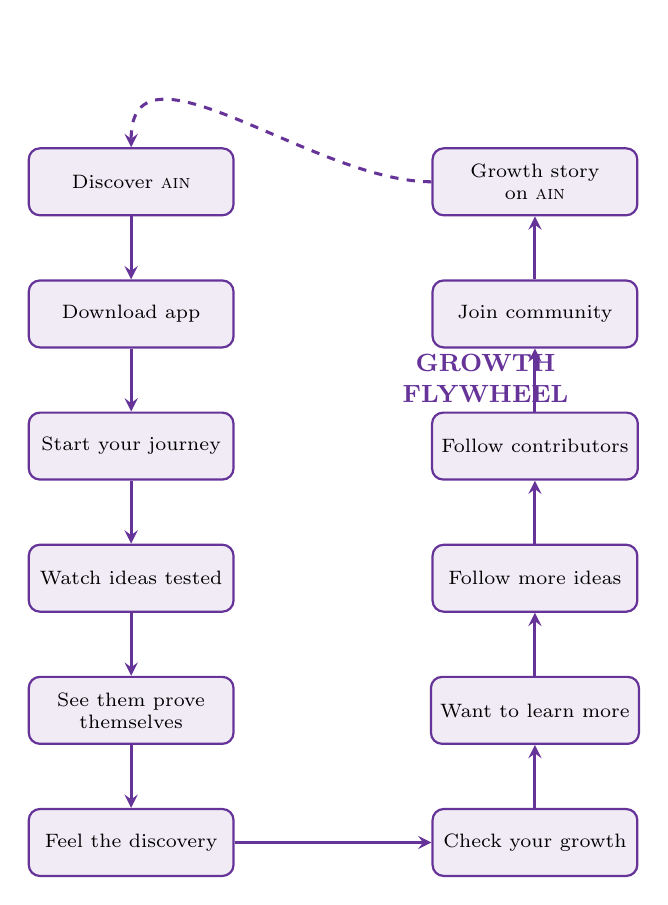
\begin{tikzpicture}[
    node distance=1.6cm,
    box/.style={rectangle, rounded corners, draw=ainpurple, thick, fill=ainpurple!10, minimum width=2.6cm, minimum height=0.85cm, align=center, font=\scriptsize},
    arrow/.style={->, thick, ainpurple, >=stealth, line width=1.1pt}
]

% Consumer flywheel (left side)
\node[box] (hear) at (0,0) {Discover \ain{}};
\node[box, below=0.8cm of hear] (download) {Download app};
\node[box, below=0.8cm of download] (portfolio) {Start your journey};
\node[box, below=0.8cm of portfolio] (notif) {Watch ideas tested};
\node[box, below=0.8cm of notif] (watch) {See them prove\\themselves};
\node[box, below=0.8cm of watch] (feel) {Feel the discovery};
\node[box, right=2.5cm of feel] (calibration) {Check your growth};
\node[box, above=0.8cm of calibration] (improve) {Want to learn more};
\node[box, above=0.8cm of improve] (more) {Follow more ideas};
\node[box, above=0.8cm of more] (follow) {Follow contributors};
\node[box, above=0.8cm of follow] (community) {Join community};
\node[box, above=0.8cm of community] (identity) {Growth story\\on \ain{}};

\draw[arrow] (hear) -- (download);
\draw[arrow] (download) -- (portfolio);
\draw[arrow] (portfolio) -- (notif);
\draw[arrow] (notif) -- (watch);
\draw[arrow] (watch) -- (feel);
\draw[arrow] (feel) -- (calibration);
\draw[arrow] (calibration) -- (improve);
\draw[arrow] (improve) -- (more);
\draw[arrow] (more) -- (follow);
\draw[arrow] (follow) -- (community);
\draw[arrow] (community) -- (identity);
\draw[arrow, dashed] (identity) to[out=180, in=90] (hear);

% Center annotation
\node[font=\small\bfseries, color=ainpurple, align=center] at (4.5, -2.5) {GROWTH\\FLYWHEEL};

\end{tikzpicture}
\end{center}

\vspace{0.3cm}

% ----------------------------------------------------------------------------
% VALUE ACCUMULATION
% ----------------------------------------------------------------------------

\begin{center}
{\Large\bfseries\color{ainpurple} Accumulated Value: Why Users Stay}
\end{center}

\vspace{0.2em}

\begin{center}
\begin{tabular}{ll}
\toprule
\textbf{Value Built on \ain{}} & \textbf{Why It's Irreplaceable} \\
\midrule
Knowledge journey history & Years of intellectual growth---your story \\
Learning Score & Proves your epistemic development---earned over time \\
Prediction track record & Your demonstrated foresight---built through experience \\
Curated follows & Your personalized discovery feed---carefully cultivated \\
Achievements & ``Early believer in X''---moments captured forever \\
Community connections & Relationships, discussions, shared exploration \\
Personalized insights & Your notification preferences, interests, focus areas \\
\rowcolor{aingold!20}
\textbf{Intellectual identity} & \textbf{``I understand AI deeply''---your growth story} \\
\bottomrule
\end{tabular}
\end{center}

\vspace{0.3em}

\begin{center}
\colorbox{ainlight}{%
\begin{minipage}{0.9\textwidth}
\centering
\vspace{0.4em}
{\bfseries The longer you use \ain{}, the richer your intellectual journey becomes.}\\
Your growth story lives here. Your learning is documented. Your insights are recognized.\\
\textit{This is an investment in yourself that compounds over time.}
\vspace{0.4em}
\end{minipage}%
}
\end{center}

\sectionline

% ----------------------------------------------------------------------------
% APP VS WEBSITE
% ----------------------------------------------------------------------------

\begin{center}
{\Large\bfseries\color{ainblue} App-First Strategy}
\end{center}

\vspace{0.2em}

\begin{multicols}{2}

\textbf{Mobile App (Primary):}
\begin{itemize}[nosep, leftmargin=1em]
    \item Notifications on ideas you follow
    \item Quick updates on the go
    \item Your journey always with you
    \item Live Deep Dive alerts
    \item Community features
    \item \textit{Where discovery happens}
\end{itemize}

\columnbreak

\textbf{Web Platform (Power Users):}
\begin{itemize}[nosep, leftmargin=1em]
    \item Deep strength gradient analysis
    \item Long-form exploration
    \item Institutional dashboards
    \item Research tools
    \item Developer console
    \item \textit{Where deep work happens}
\end{itemize}

\end{multicols}

% ============================================================================
% PAGE 4
% ============================================================================

\newpage

\begin{center}
{\fontsize{26}{32}\selectfont\bfseries\color{ainblue} The Complete Flywheel}
\end{center}

\sectionline

\vspace{0.3em}

\begin{center}
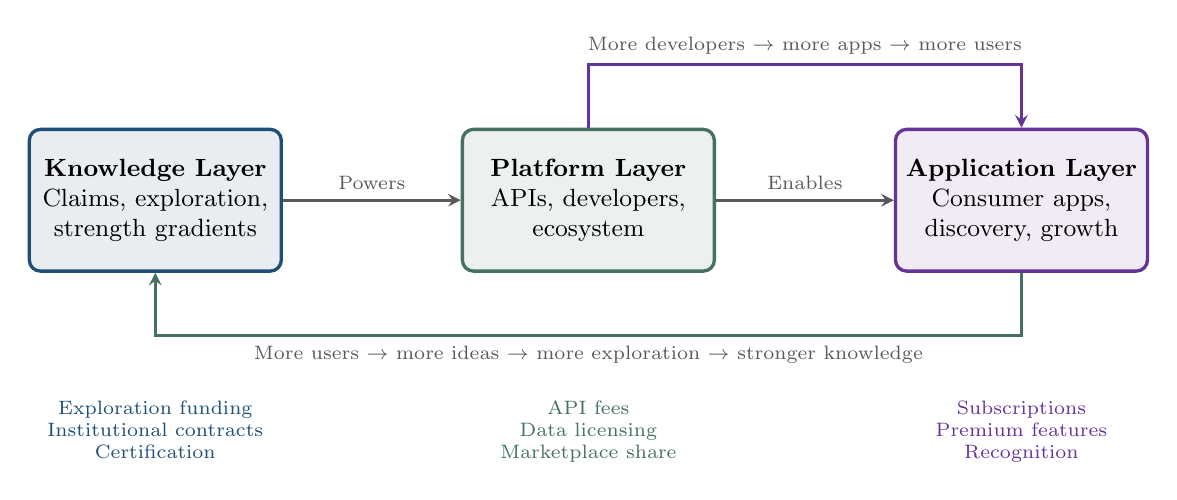
\begin{tikzpicture}[
    node distance=1.2cm and 2cm,
    layer/.style={rectangle, rounded corners, draw=#1, line width=1.2pt, fill=#1!10, minimum width=3.2cm, minimum height=1.8cm, align=center, font=\small},
    arrow/.style={->, thick, aingray, >=stealth, line width=1pt}
]

% Three layers
\node[layer=ainblue] (truth) at (0,0) {\textbf{Knowledge Layer}\\Claims, exploration,\\strength gradients};

\node[layer=aingreen] (platform) at (5.5,0) {\textbf{Platform Layer}\\APIs, developers,\\ecosystem};

\node[layer=ainpurple] (apps) at (11,0) {\textbf{Application Layer}\\Consumer apps,\\discovery, growth};

% Arrows between layers
\draw[arrow] (truth) -- (platform) node[midway, above, font=\scriptsize] {Powers};
\draw[arrow] (platform) -- (apps) node[midway, above, font=\scriptsize] {Enables};

% Feedback loops
\draw[arrow, aingreen] (apps.south) -- ++(0,-0.8) -| (truth.south) 
    node[pos=0.25, below, font=\scriptsize, text=aingray] {More users $\rightarrow$ more ideas $\rightarrow$ more exploration $\rightarrow$ stronger knowledge};

\draw[arrow, ainpurple] (platform.north) -- ++(0,0.8) -| (apps.north)
    node[pos=0.25, above, font=\scriptsize, text=aingray] {More developers $\rightarrow$ more apps $\rightarrow$ more users};

% Revenue indicators
\node[below=1.5cm of truth, font=\scriptsize, align=center, text=ainblue] {Exploration funding\\Institutional contracts\\Certification};
\node[below=1.5cm of platform, font=\scriptsize, align=center, text=aingreen] {API fees\\Data licensing\\Marketplace share};
\node[below=1.5cm of apps, font=\scriptsize, align=center, text=ainpurple] {Subscriptions\\Premium features\\Recognition};

\end{tikzpicture}
\end{center}

\vspace{0.5em}

\begin{center}
\colorbox{ainblue}{%
\begin{minipage}{0.95\textwidth}
\centering
\vspace{0.5em}
{\large\bfseries\color{white} The Reinforcing Loop}\\[0.4em]
{\color{white}
\textbf{Discovery} drives consumer adoption $\rightarrow$ More users means more ideas explored\\
$\rightarrow$ Better gradients means stronger \textbf{knowledge} $\rightarrow$ Institutions invest\\
$\rightarrow$ High-profile ideas create \textbf{inspiring journeys} $\rightarrow$ Developers build apps $\rightarrow$ More discovery\\
$\rightarrow$ \textbf{Network effects} compound $\rightarrow$ \textbf{Canonical status} $\rightarrow$ The place where knowledge lives
}
\vspace{0.5em}
\end{minipage}%
}
\end{center}

\sectionline

% ----------------------------------------------------------------------------
% COMPLETE MONETIZATION
% ----------------------------------------------------------------------------

\begin{center}
{\Large\bfseries\color{ainblue} Complete Value Capture}
\end{center}

\vspace{0.2em}

\begin{center}
\begin{small}
\begin{tabular}{lllll}
\toprule
\textbf{Layer} & \textbf{Revenue Stream} & \textbf{Model} & \textbf{Scale} & \textbf{Margin} \\
\midrule
\rowcolor{ainblue!10}
Knowledge & Exploration funding fees & 0.5--2\% coordination & $\propto$ activity & Very high \\
\rowcolor{ainblue!10}
Knowledge & Institutional partnerships & Annual/custom & Enterprise & High \\
\rowcolor{ainblue!10}
Knowledge & ``\ain{}-verified'' certification & Per-cert + annual & Trust-driven & Very high \\
\midrule
\rowcolor{aingreen!10}
Platform & API usage fees & Per-call / tiered & Developer adoption & High \\
\rowcolor{aingreen!10}
Platform & Data licensing & Subscription & Research/enterprise & High \\
\rowcolor{aingreen!10}
Platform & Contributor marketplace & Revenue share & Ecosystem & Medium \\
\rowcolor{aingreen!10}
Platform & Premium SDKs/tools & Subscription & Power developers & High \\
\midrule
\rowcolor{ainpurple!10}
Application & Premium subscriptions & Monthly/annual & Consumer scale & Medium \\
\rowcolor{ainpurple!10}
Application & Advanced features & In-app purchases & Power users & High \\
\rowcolor{ainpurple!10}
Application & Verified contributor badges & One-time + renewal & Recognition & Very high \\
\rowcolor{ainpurple!10}
Application & Thoughtful sponsorships & Selective partnerships & Brand alignment & Medium \\
\bottomrule
\end{tabular}
\end{small}
\end{center}

\vspace{0.3em}

\begin{center}
\textit{Every layer creates value. Every layer captures value. Every layer reinforces the others.}
\end{center}

% ============================================================================
% PAGE 5
% ============================================================================

\newpage

\begin{center}
{\fontsize{26}{32}\selectfont\bfseries\color{ainblue} Why This Succeeds}
\end{center}

\sectionline

\vspace{0.3em}

% ----------------------------------------------------------------------------
% PHILOSOPHICAL FOUNDATION
% ----------------------------------------------------------------------------

\begin{center}
{\Large\bfseries\color{ainblue} Philosophical Foundation}
\end{center}

\vspace{0.2em}

\begin{center}
\begin{small}
\begin{tabularx}{0.95\textwidth}{lX}
\toprule
\textbf{Thinker} & \textbf{Contribution to \ain{}} \\
\midrule
\textbf{Popper} & Knowledge grows stronger through rigorous examination. \ain{} makes this possible at scale. \\
\textbf{Lakatos} & Ideas form networks; some core, some evolving. Strength gradients capture this structure. \\
\textbf{Quine} & No idea tested in isolation; webs of understanding. Gradients show interdependence. \\
\textbf{Peirce} & Truth = what inquiry converges on under good conditions. \ain{} creates those conditions. \\
\textbf{Habermas} & Good discourse: openness, reason, no coercion. \ain{} embodies these principles. \\
\bottomrule
\end{tabularx}
\end{small}
\end{center}

\vspace{0.2em}

\begin{center}
{\bfseries \ain{} is 90 years of philosophy of science, finally given infrastructure to flourish.}
\end{center}

\sectionline

% ----------------------------------------------------------------------------
% INFRASTRUCTURE ANALOGY
% ----------------------------------------------------------------------------

\begin{center}
{\Large\bfseries\color{ainblue} The Next Layer of Human Infrastructure}
\end{center}

\vspace{0.2em}

\begin{center}
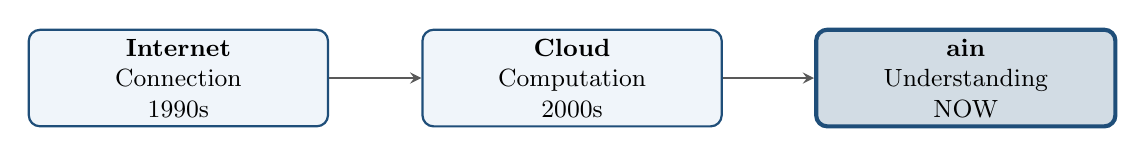
\begin{tikzpicture}[
    layer/.style={rectangle, rounded corners, draw=ainblue, thick, fill=ainlight, minimum width=3.8cm, minimum height=1cm, align=center, font=\small},
    arrow/.style={->, thick, aingray, >=stealth}
]

\node[layer] (l1) at (0,0) {\textbf{Internet}\\Connection\\1990s};
\node[layer] (l2) at (5,0) {\textbf{Cloud}\\Computation\\2000s};
\node[layer, fill=ainblue!20, draw=ainblue, line width=1.5pt] (l3) at (10,0) {\textbf{\ain{}}\\Understanding\\NOW};

\draw[arrow] (l1) -- (l2);
\draw[arrow] (l2) -- (l3);

\end{tikzpicture}
\end{center}

\vspace{0.2em}

\begin{center}
\textit{The internet connected us. Cloud empowered us. \ain{} helps us understand together.}
\end{center}

\sectionline

% ----------------------------------------------------------------------------
% MOAT & NETWORK EFFECTS
% ----------------------------------------------------------------------------

\begin{center}
{\Large\bfseries\color{ainblue} Network Effects \& Sustainable Advantage}
\end{center}

\vspace{0.2em}

\begin{multicols}{2}

\textbf{Network Effects (Each Layer):}
\begin{itemize}[nosep, leftmargin=1em]
    \item Knowledge: More ideas $\rightarrow$ richer gradients
    \item Platform: More developers $\rightarrow$ more tools
    \item Apps: More users $\rightarrow$ vibrant community
    \item Cross-layer: Each strengthens the others
\end{itemize}

\columnbreak

\textbf{Sustainable Advantage:}
\begin{itemize}[nosep, leftmargin=1em]
    \item \textbf{Accumulated understanding}: Years of knowledge
    \item \textbf{Contributor reputation}: Earned through contribution
    \item \textbf{User journeys}: Growth stories documented
    \item \textbf{Developer ecosystem}: Integration investment
    \item \textbf{Certification standard}: Industry adoption
    \item \textbf{Canonical status}: Where understanding lives
\end{itemize}

\end{multicols}

\sectionline

% ----------------------------------------------------------------------------
% CLOSING
% ----------------------------------------------------------------------------

\vspace{0.5em}

\begin{center}
\colorbox{ainblue}{%
\begin{minipage}{0.95\textwidth}
\centering
\vspace{0.6em}
{\Large\bfseries\color{white} The Vision}\\[0.5em]
{\large\color{white} 
\ain{} is \textbf{knowledge infrastructure}---the next layer after connection and computation.\\[0.3em]
We steward the \textbf{Knowledge Layer}: the trusted foundation where ideas prove themselves.\\[0.3em]
We open the \textbf{Platform Layer}: APIs, SDKs, data feeds---anyone can build with us.\\[0.3em]
We create the \textbf{Application Layer}: discovery, growth, community---where learning comes alive.\\[0.5em]
Three layers. All creating value. All reinforcing. All built to last.\\[0.3em]
\textbf{We're building the place where ideas prove themselves,\\knowledge grows stronger, and understanding deepens together.}
}
\vspace{0.6em}
\end{minipage}%
}
\end{center}

\vspace{0.8em}

\begin{center}
{\large\itshape 
``Where ideas prove themselves.\\
Where knowledge grows stronger.\\
Where understanding deepens together.''}
\end{center}

\vspace{0.5em}

\begin{center}
\colorbox{aingreen!20}{%
\begin{minipage}{0.7\textwidth}
\centering
\vspace{0.4em}
{\large\bfseries The Tagline}\\[0.2em]
{\Large\itshape ``The forge where knowledge grows stronger.''}
\vspace{0.4em}
\end{minipage}%
}
\end{center}

\vspace{1em}

\begin{center}
{\color{aingray}\small Bernd J. Wuebben\quad$\bullet$\quad\today\quad$\bullet$\quad v0.6}
\end{center}

\end{document}
